\documentclass[12pt,a4paper]{article}
\usepackage{geometry}
\usepackage[numbers]{natbib}
\usepackage{amssymb, amsmath}
\usepackage{graphicx}
\usepackage{grffile}
\graphicspath{{../Figures/}}
\usepackage{gensymb}
\usepackage[font=small]{caption}
\usepackage[utf8]{inputenc}
\usepackage[english]{babel}
\usepackage{fancyhdr}
\usepackage[raggedright]{titlesec}
\usepackage{subcaption}
\usepackage{multirow}
\usepackage{dirtytalk}
\usepackage{framed}
\usepackage[pdftex,breaklinks]{hyperref}
\hypersetup{
  colorlinks   = true, %Colours links instead of ugly boxes
  urlcolor     = green, %Colour for external hyperlinks
  linkcolor    = blue, %Colour of internal links
  citecolor   = red %Colour of citations
}


\begin{document}
\author{Katrina Ashton}


\pagestyle{fancy}
\fancyhf{}
\rhead{\thepage}
\lhead{u5586882}

\section{What I've done}
\begin{itemize}
\item{Worked with Jean-Luc to get Vicon-assisted autonomous flight working and learnt how to use it.}
\item{Flew quad and collected data.}
\item{Updated draft of mid term report.}
\end{itemize}

\section{Parts of report to look at}
\begin{itemize}
\item{Nothing changed since last week}
\end{itemize}

\section{Questions}
\begin{itemize}
\item
\end{itemize}

\section{Comments}
\begin{itemize}
\item I'll probably do another round of data acquisition with a slower movement speed at some point this week.
\end{itemize}

\section{Experiments}
\section{Data acquisition}
\textbf{Purpose} \\
To use the RealSense camera mounted to my quadcopter to capture point clouds representing a scene. These point clouds will be then be registered to recover a 3D model of the scene.
\\\\
Thus each frame must have enough overlap with the previous one in order to register them. Also, ground truth data for the scene and quadcopter position are required in order to verify if the scene has been accurately represented.
\\\\
\textbf{Set-up} \\
The scene is made up of four boxes, arranged as shown in Figure \ref{f: e1 r2 setup}. These are place in the center of the room, which is currently set as the origin of the Vicon assisted velocity controller program. The quadcopter is programmed to hover for 30 seconds and then fly in a circle of radius 1.2m around the origin, with a height of 1.2m. It flies around twice, taking 40 seconds each time. Afterwards it will hover in place and then descend. 
\begin{figure}[h]
	\centering
    \includegraphics[width=50mm, trim =110mm 70mm 110mm 110mm, clip]{setup/IMG_20180518_140507.jpg}
	\caption{Set-up of scene for first flight experiment}
	\label{f: e1 r2 setup}
\end{figure}

\noindent
\textbf{Method} \\
The quadcopter is flown using a Vicon assisted velocity controller program. In order for this program to work the following steps must be completed:
\begin{enumerate}
\item Turn on Vicon system.
\item Set-up scene and quadcopter. The quadcopter should be facing the scene 1.2m back, it should also be pointing forwards as defined by the Vicon system.
\item Ensure that the quadcopter is showing up on the Vicon system. Tune the strobing and threshold if necessary to remove reflected landmarks. If tuning is not sufficient then try using electrical tape to cover reflective parts of the quadcopter.
\item Turn on and arm the quadcopter.
\item Connect ground station computer to the Vicon via ethernet and ensure that the radio is plugged in and connected to its pair on the quadcopter.
\item Run \verb|roslaunch mavros px4.launch|
\item In a new terminal run \verb|roslaunch vicon_bridge vicon.launch|.
\item In a new terminal run \verb|sh connect_tx2_realsense.sh| (ensure that the TX2 and ground station computer are connected to the same network).
\item In the ssh terminal, create a new terminal using \verb|gnome-terminal| and \verb|cd| to the SSD card. From there run the data acquisition code with \verb|./cpp-pointcloud-save|
\item In the original ssh terminal, run \verb|sh run_vicon.sh|. This will open up a number of terminal windows. The last one should say something along the lines of "in hover mode". This has started the velocity controller, so the quadcopter needs to be launched within 30 seconds.
\item Use the controller to arm the quadcopter and flick it into autonomous mode to launch.
\item Start the data acquisition code while the quadcopter is still hovering.
\item Wait until the quadcopter finishes doing two circles and the stop the data acquisition code while it is hovering. Only attempt to land or disarm the quad in an emergency.
\item Once the quadcopter has hovered in place for a bit it will descend. Once it has reached the ground the controller should be switched back into manual mode and then used to disarm the quadcopter.
\end{enumerate}

\noindent
\textbf{Results} \\
\begin{figure}[h]
	\centering
	\begin{subfigure}[t]{0.5\textwidth}
	\centering
    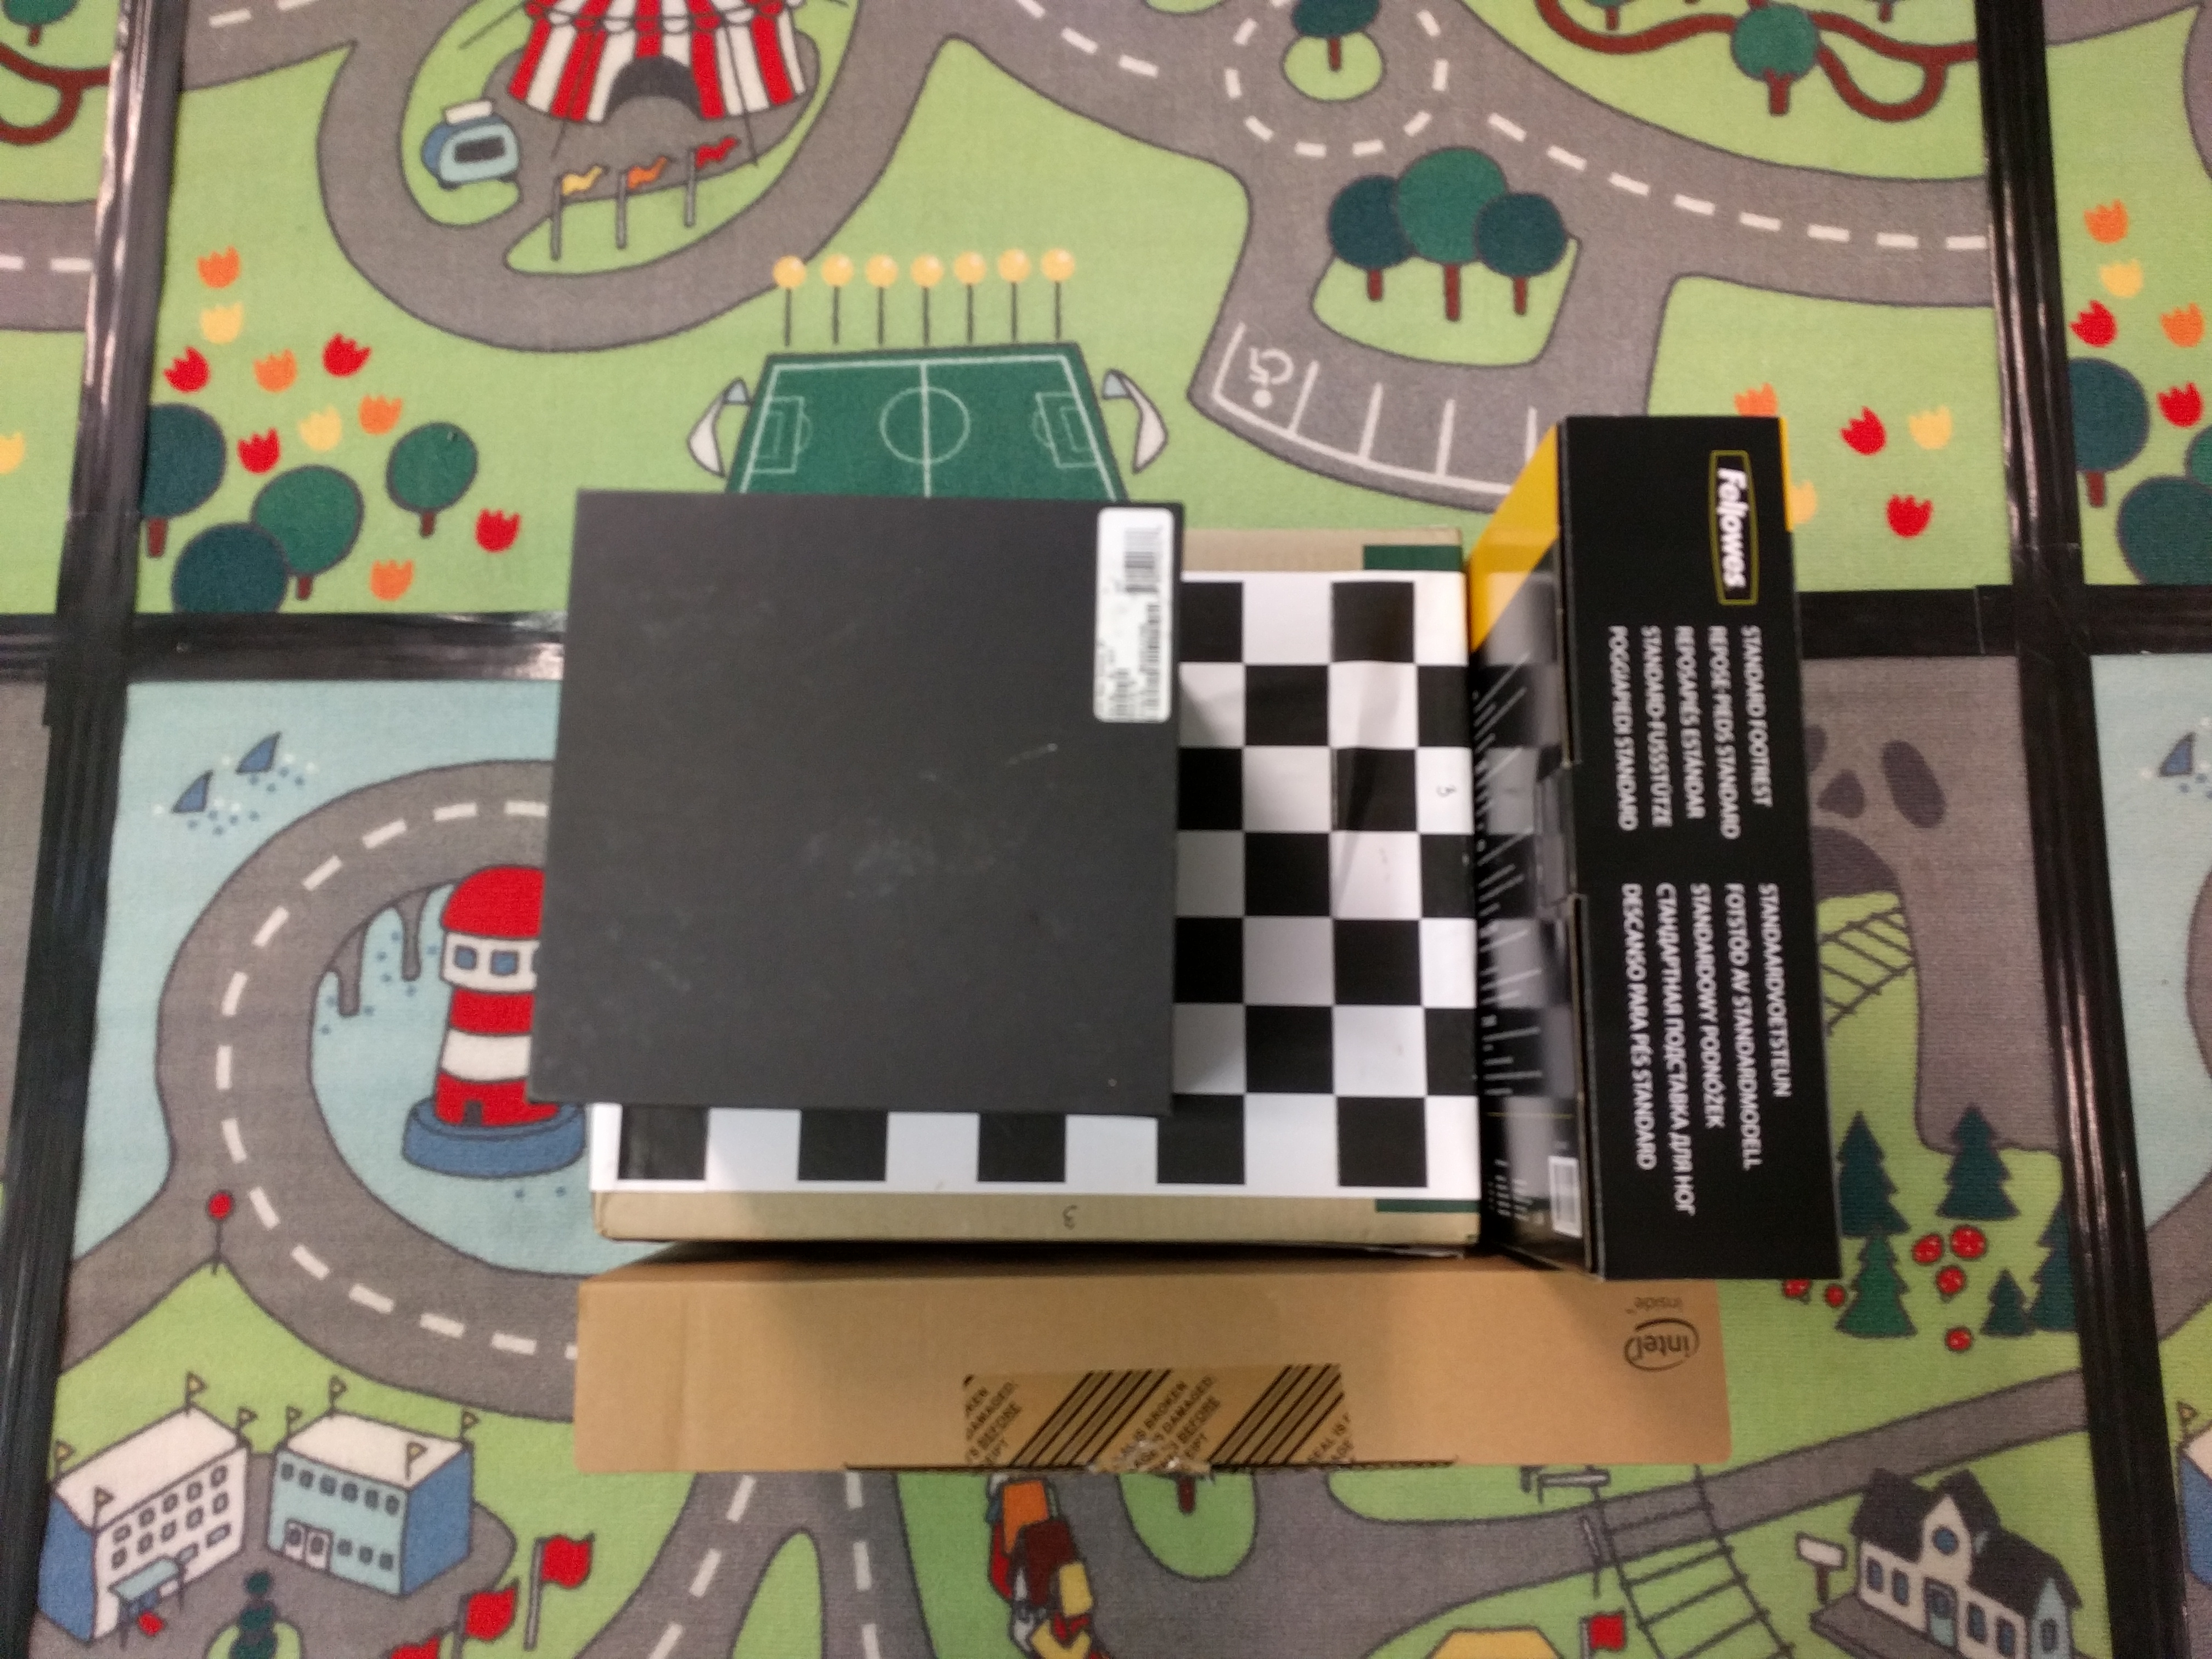
\includegraphics[width=50mm, trim =110mm 70mm 110mm 110mm, clip]{setup/IMG_20180518_142317.jpg}
	\caption{Top-down view of scene}
	\label{f: e1 r2 setup}
	\end{subfigure}
	\\
	\begin{subfigure}[t]{0.5\textwidth}
	\centering
    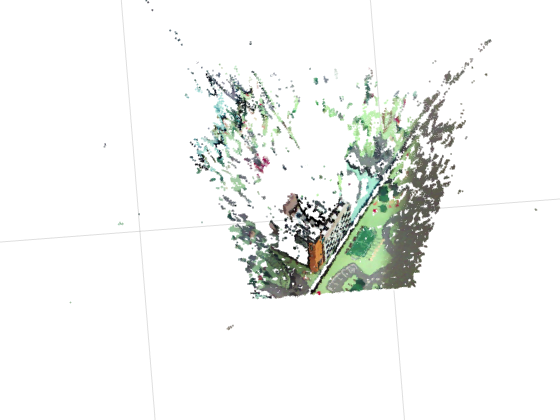
\includegraphics[width=70mm, trim =20mm 25mm 15mm 5mm, clip]{run2_frame50.png}
	\caption{Example of point cloud from a single frame}
	\label{f: e1 r2 50}
	\end{subfigure}%
	~
	\begin{subfigure}[t]{0.5\textwidth}
	\centering
    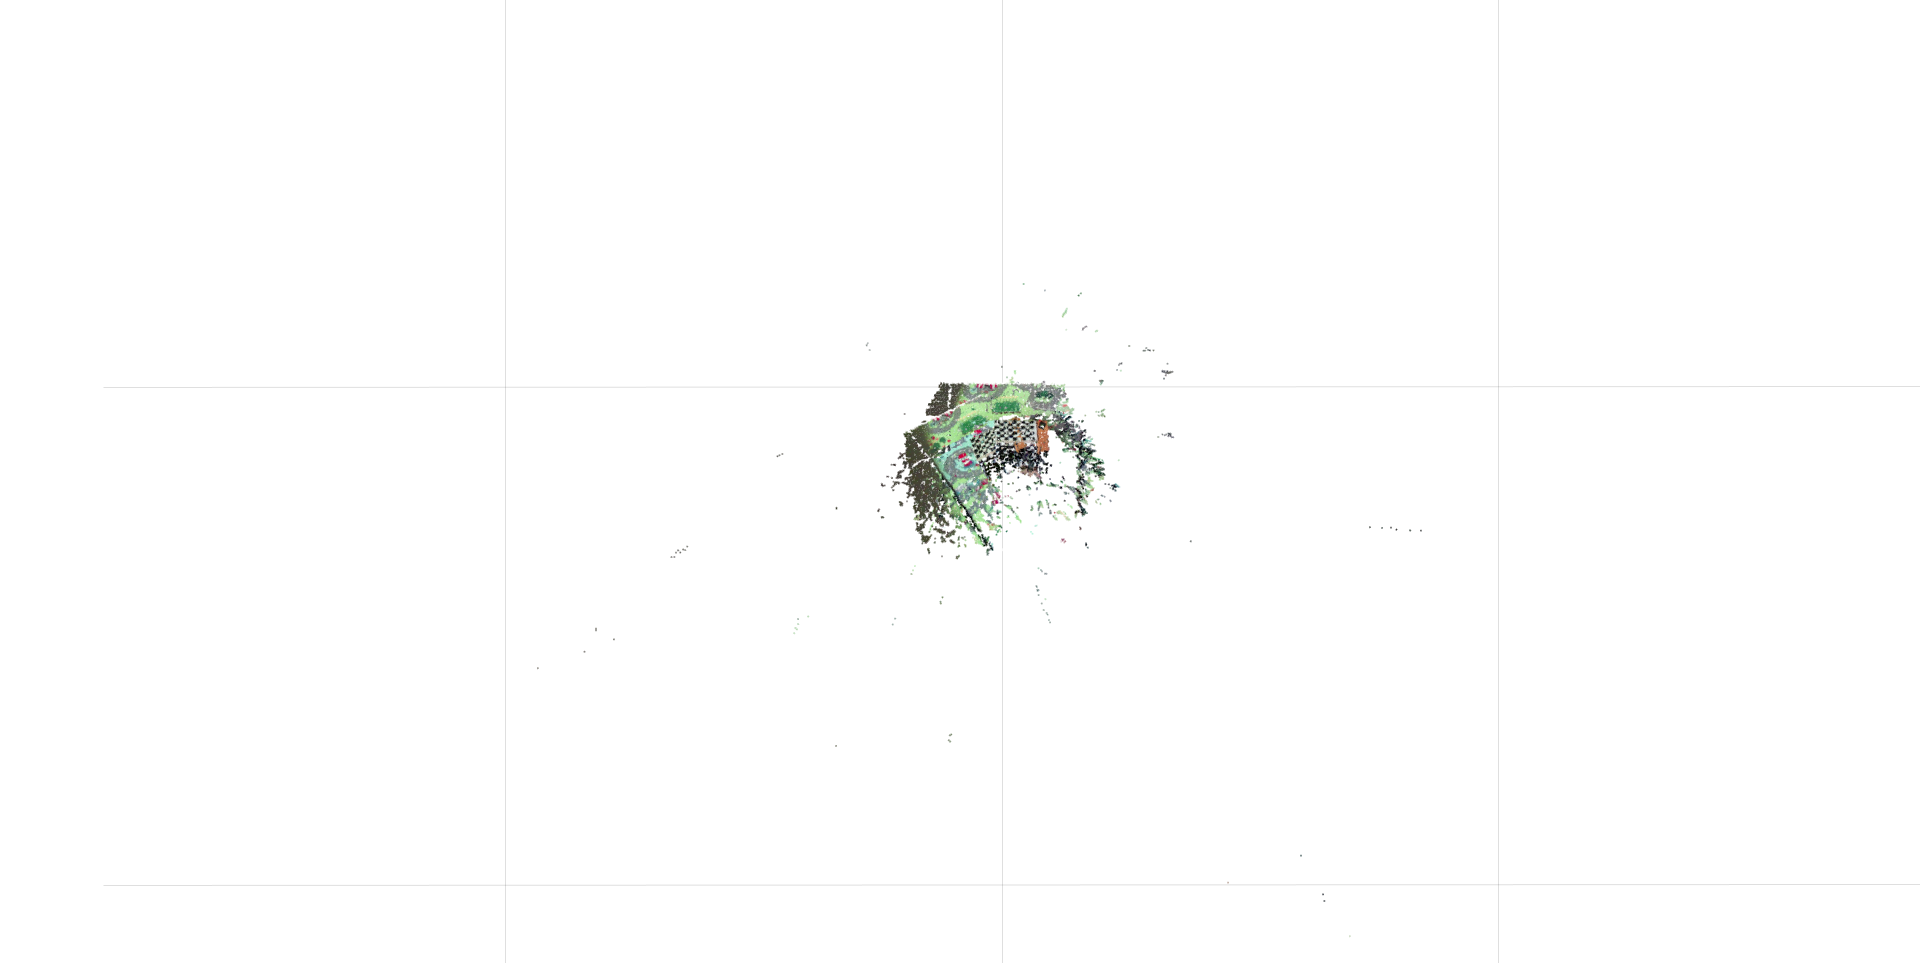
\includegraphics[width=70mm, trim =200mm 100mm 200mm 90mm, clip]{run2_updatedworld.png}
	\caption{Point cloud registered using MATLAB}
	\label{f: e1 r2 all}
	\end{subfigure}
	\caption{Comparison of point clouds to scene for first flying experiment.}
	\label{f: e1 r2}
\end{figure}

\noindent
Many of the individual frames only capture part of the scene (see Figure \ref{f: e1 r2 50}). When registering the data using MATLAB's pcregistericp method the resulting point cloud is still missing points in some areas, and it does not seem to have done a good job aligning the point clouds for the checkered box (see Figure \ref{f: e1 r2 all} compared to \ref{f: e1 r2 setup}).
\\\\
The gap in the point cloud is at the back of the boxes, which cannot be seen while the quadcopter is hovering. This suggests that the quadcopter may not be capturing enough data while it is flying in the circle to register it properly.
\\\\
\textbf{Conclusion}
It would be good to fly the quadcopter slightly more slowly while capturing the data and seeing if this results in a better registered point cloud model.
\\\\
\newpage
From last week:
\section{Testing RealSense with Vicon}
\textbf{Purpose} \\
The RealSense camera and Vicon system both use IR. Thus it is possible that the Vicon system interferes with the RealSense's depth measurements. The purpose of this experiment is to determine if this interference occurs or not.
\\\\
\textbf{Set-up} \\
The RealSense camera is set-up pointing at a number of objects lying on the ground of the flying space. It is positioned in the groove of the white box. It stays relatively still but both the box and the RealSense itself are sensitive to bumps.
\\\\
The RealSense is connected to the TX2 (with orbitty board), and then SSHed to via an Ethernet cable. 
\\\\
\textbf{Method} \\
The camera remains still while point clouds are captured for about 5 seconds. The data collection program is then stopped. 
\\\\
For some reason the code wasn't letting the data collection program be re-run through SSH after it was canceled without restarting the TX2 (I did not have this issue with the TX1 which I connected to directly). Thus the TX2 was restarted by disconnecting and reconnecting the power (taking care not to bump the camera). Before the power was reconnected, the SD card was also removed from the TX2 and inserted into a laptop. The captured point clouds were moved to a separate folder so that it would be clear under which conditions they were captured.
\\\\
The Vicon system was then activated and the above procedure repeated (but without reconnecting the power for the TX2 at the end).
\\\\
\textbf{Results} \\
	\begin{figure}[h]
		\centering
		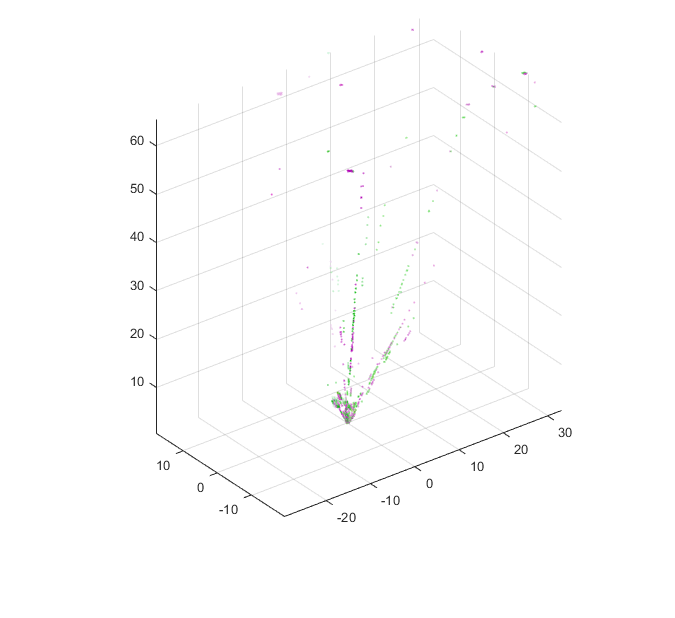
\includegraphics[height=50mm, trim = 20mm 20mm 20mm 20mm, clip]{first_frame_compare.png}
		\caption{Comparison of first point cloud with (green) and without (purple) Vicon on. Registering the point clouds gives a sum-squared difference of 0.3223 to I, with rmse 0.5990 for the registration.}
		\label{f: vicon first frame}
	\end{figure}

	\begin{figure}[h]
		\centering
		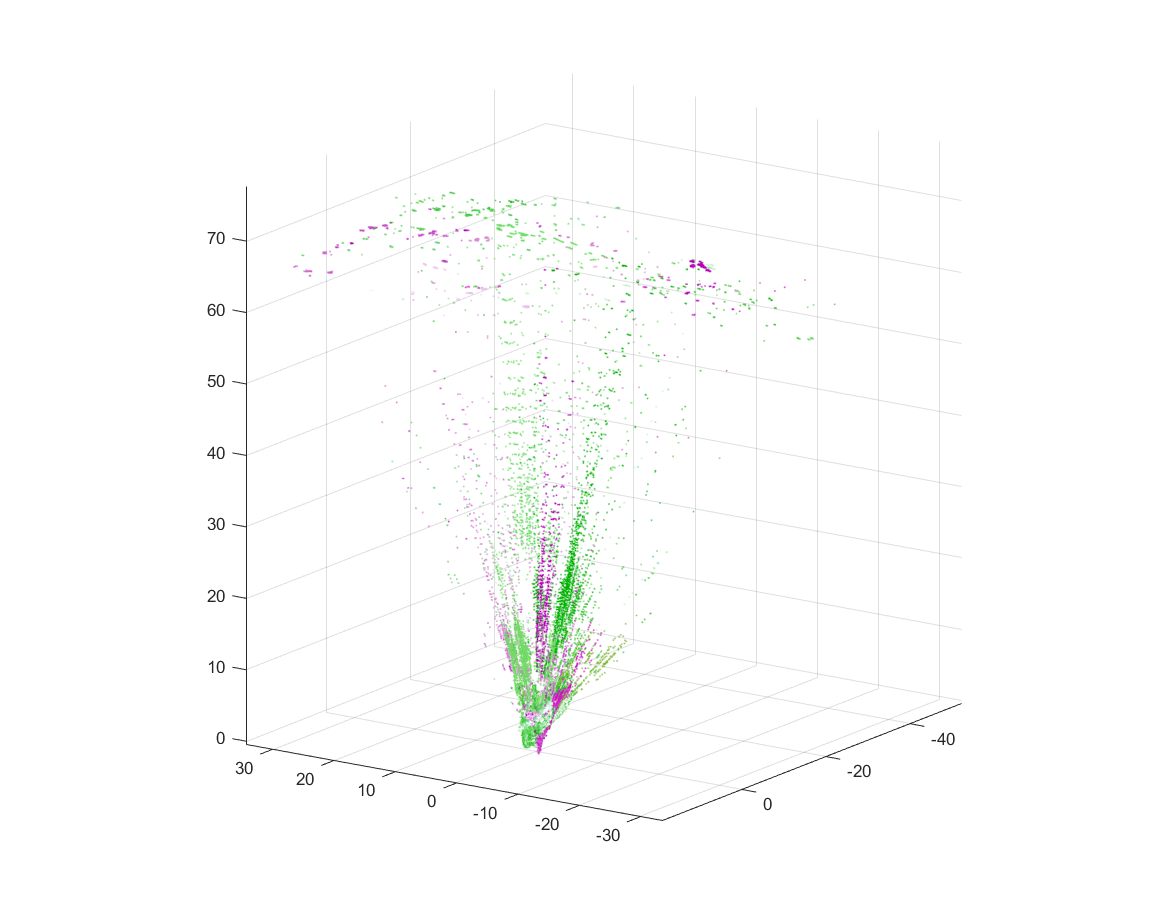
\includegraphics[height=50mm, trim = 20mm 20mm 20mm 20mm, clip]{full_compare.png}
		\caption{Comparison of registered point clouds with (green) and without (purple) Vicon on. Registering the point clouds gives a sum-squared difference of 0.0094 to I, with rmse 0.4770 for the registration.}
		\label{f: vicon all frame}
	\end{figure}
\noindent
There are only small differences between the point clouds for the scene with and without the Vicon. It is possible that these could have been caused by the camera moving slightly as it was not held securely in place and so would have been susceptible to bumps. There will also be noise present. This is supported by the fact that the difference from the identity and rmse error for the registration were both smaller for the full point cloud rather than just the first frame.
\\\\
\textbf{Conclusion} \\
The Vicon does not appear to significantly affect the RealSense's ability to capture depth data. Thus we will be able to use both at the same time for the data capture.

\newpage
\section{Testing RealSense for different movement speeds}
\textbf{Purpose} \\
In order to register point clouds there needs to be some degree of overlap between them. Thus to get usable data I must investigate how quickly I can move the camera while still obtaining frames with enough overlap. In addition, depending on how the point clouds are captured and processed, moving the camera too quickly may result in motion blur which should be avoided. The purpose of this experiment is to determine the fastest speed I can move the RealSense camera in while still allowing getting overlap between point clouds and without getting motion blur.
\\\\
\textbf{Set-up} \\
Two strips of tape are placed on the (straight) edge of a desk about 60cm apart.
\\\\
The RealSense is connected to the TX2 (with orbitty board), and then SSHed to via an Ethernet cable. 
\\\\
\textbf{Method} \\
Camera is held with the end at the edge of the left piece of tape, sitting on the edge of the table. The data capture program is started while the camera is held still for 4 seconds (letting the exposure, etc. settle). The camera is then moved at a slow speed along the edge of the table to the other end of the tape, after which the data capture program is immediately canceled. The camera was moved by hand, so there was likely variation in the movement speed.
\\\\
As with the Vicon test, the TX2 had to be restarted between tests. The data was also moved to a separate folder after each test.
\\\\
The above was repeated with medium-speed camera movement and then again with fast movement.
\\\\
\textbf{Results} \\
	\begin{figure}[h]
		\centering
		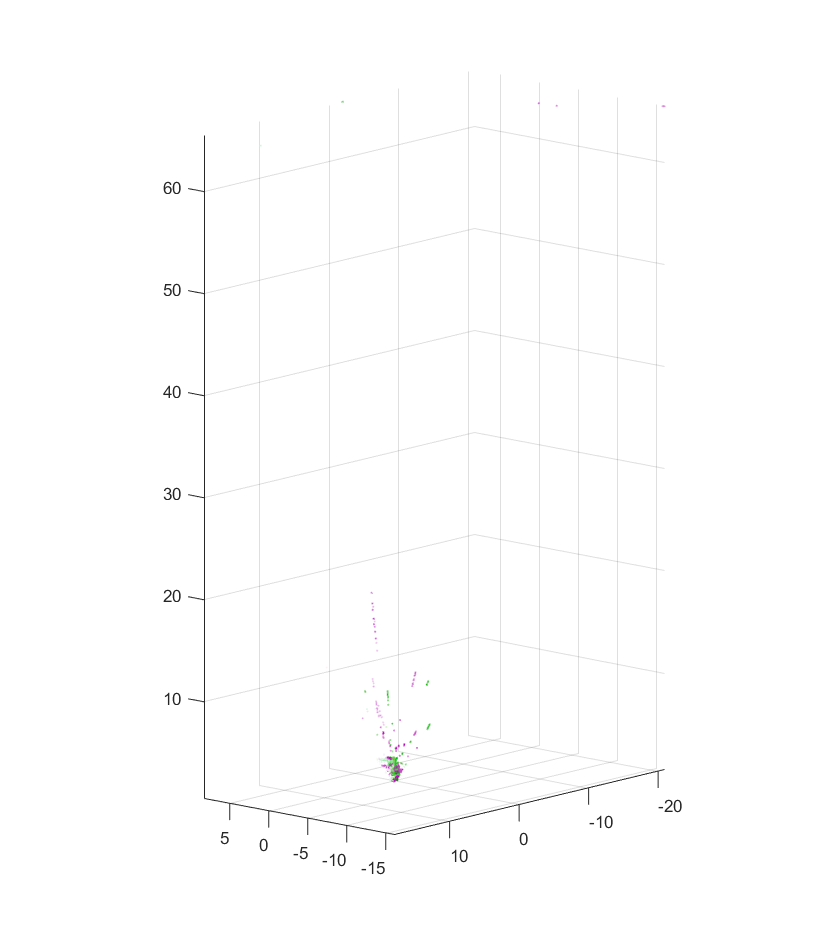
\includegraphics[height=50mm, trim = 20mm 10mm 20mm 140mm, clip]{slow_med.png}
		\caption{Comparison of middle point cloud for a camera that is moving slowly (green) and at a medium speed (purple). Registering the point clouds gives a sum-squared difference of 0.1226 to I, with rmse 0.2146 for the registration.}
		\label{f: slow v med}
	\end{figure}

	\begin{figure}[h]
		\centering
		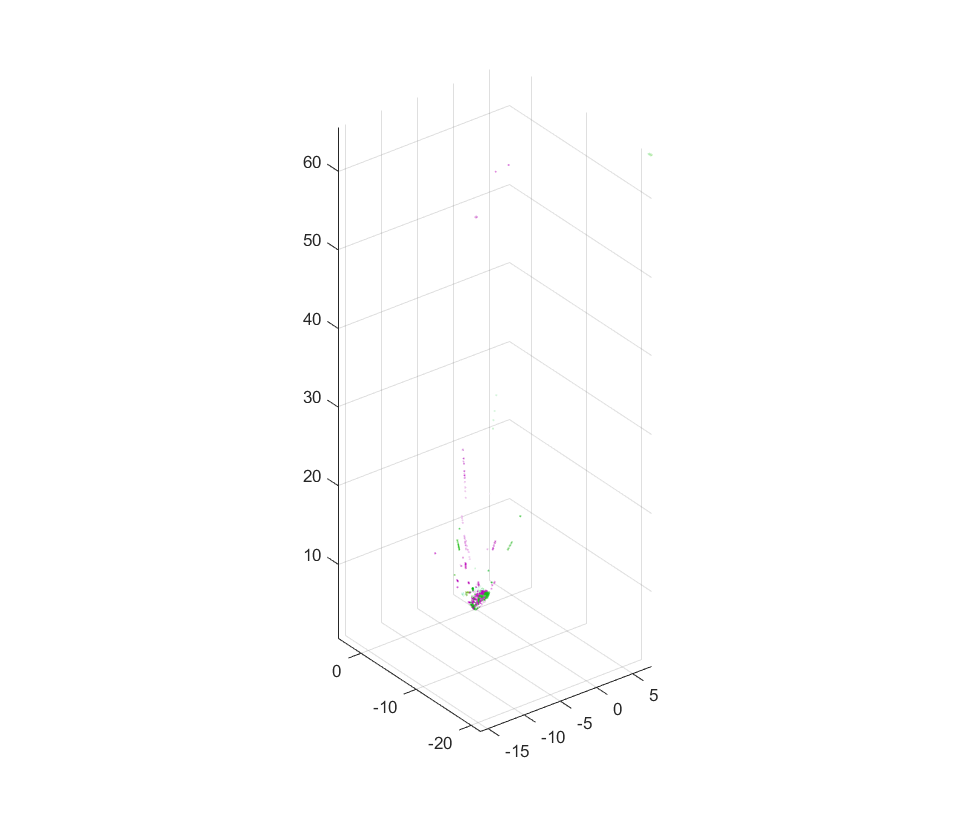
\includegraphics[height=50mm, trim = 20mm 10mm 20mm 100mm, clip]{slow_fast.png}
		\caption{Comparison of middle point cloud for a camera that is moving slowly (green) and quickly (purple). Registering the point clouds gives a sum-squared difference of 0.1932 to I, with rmse 0.1690 for the registration.}
		\label{f: slow v med}
	\end{figure}
\noindent
It was checked that all of point clouds could be registered for all of the different speeds. All of them were able to be registered.
\\\\
There is a difference between the point cloud obtained during the slow movement and during the medium speed movement, and a larger difference between the slow and fast movement. This difference is, however, relatively small. Thus it could be caused by noise and/or the camera not being at the same position when the data was captured.
\\\\
\textbf{Conclusion} \\
It seems like the camera can be moved relatively quickly while still capturing usable data. However more trials need to be performed in order to get more reliable results. The camera was moved by hand for this experiment, so the motion was not uniform and the exact speed is unknown. Ideally the experiment would use equipment that would allow for uniform motion.
\\\\
Only 3 point clouds were captured for the fast motion, so if possible future trials should also use a longer distance so that more point clouds can be obtained. This is important for verifying that there is enough overlap between point clouds for registration.

\end{document}